\documentclass{standalone}
\usepackage{tikz}

\begin{document}
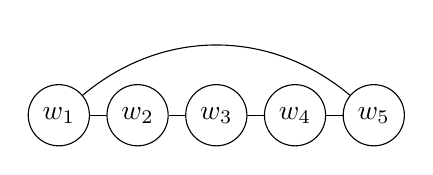
\begin{tikzpicture}
\node[shape=circle,draw=black] at (0, 0) (w1) {$w_1$};
\node[shape=circle,draw=black] at (1, 0) (w2) {$w_2$};
\node[shape=circle,draw=black] at (2, 0) (w3) {$w_3$};
\node[shape=circle,draw=black] at (3, 0) (w4) {$w_4$};
\node[shape=circle,draw=black] at (4, 0) (w5) {$w_5$};
\draw (w1) -- (w2);
\draw (w2) -- (w3);
\draw (w3) -- (w4);
\draw (w4) -- (w5);
\draw (w5) to [out=140,in=40] (w1);
\end{tikzpicture}
\end{document}
